% !TeX root = ../pythonTutorial.tex
\chapter*{Vorwort}
Das vom Stifterverband gef�rderte Projekt \glqq Informatik studieren in der digitalen Gesellschaft (InfoStuDi)\grqq{}
erprobt und evaluiert neue Lehr-, Lern- und Pr�fungsformen in den Informatik-Studieng�ngen im Fachbereich Informatik und Mikrosystemtechnik der Hochschule Kaiserslautern.
Studieng�nge an einer Hochschule f�r
angewandte Wissenschaften bereiten die Studierenden auf die sp�tere Arbeitswelt vor.
Diese Arbeitswelt
wird von zeitlich und �rtlich ungebundenem T�tigkeiten gepr�gt sein.

Im Teilprojekt \glqq Collaborative Writing\grqq{} wurde eine neue Form einer Lehrveranstaltung erprobt.
Ein Team aus Studierenden und Lehrenden verfasst ein Dokument zu einem Thema der Informatik.
Dabei wird neben der Produktion von Texten auch Software entstehen.
Die Produktion des vorliegenden Dokuments
zum Thema Python wurde wie ein gro�es agiles Software-Projekt organisiert.
Drei Sprints wurden durchgef�hrt, das Team organisierte sich selbst. Werkzeuge wie \LaTeX{}, Git oder Jenkins wurden eingesetzt.
Die Studierenden waren nicht nur Autoren, sondern auch Fachlektoren, Software-Entwickler und f�r die Qualit�t des Gesamtergebnisses mit verantwortlich.

Dieses Projekt w�re nicht zustande gekommen ohne die Studierenden, die sich auf dieses Abenteuer im Rahmen
der Lehrveranstaltung \glqq Aktuelle Themen aus Forschung und Praxis\grqq{} im Masterstudiengang Informatik eingelassen haben. An dieser Stelle ein herzliches \glqq Danke Sch�n!\grqq{} f�r das Vertrauen und den Mut, sich auf diese Form einer
Lehrveranstaltung einzulassen.
Miriam Lohm�ller brachte ihre Erfahrung aus dem Verlagswesen ein und hat die von den Studierenden verfassten
Texte lektoriert. Fabian Kalweit hat das fachliche Lektorat unterst�tzt und insbesondere das Backend in GitHub
organisiert und gestaltet.
\vspace{\baselineskip}
\begin{flushright}\noindent
Zweibr�cken, im Februar 2019\hfill

\hfill {\it Manfred  Brill}
\end{flushright}
\pagebreak
%\section*{Das Team}
%Gruppenbild mit Dame -- das Team nach dem letzten Sprint Meeting am 31.~Januar~2019.

\begin{figure}[ht]
\centering
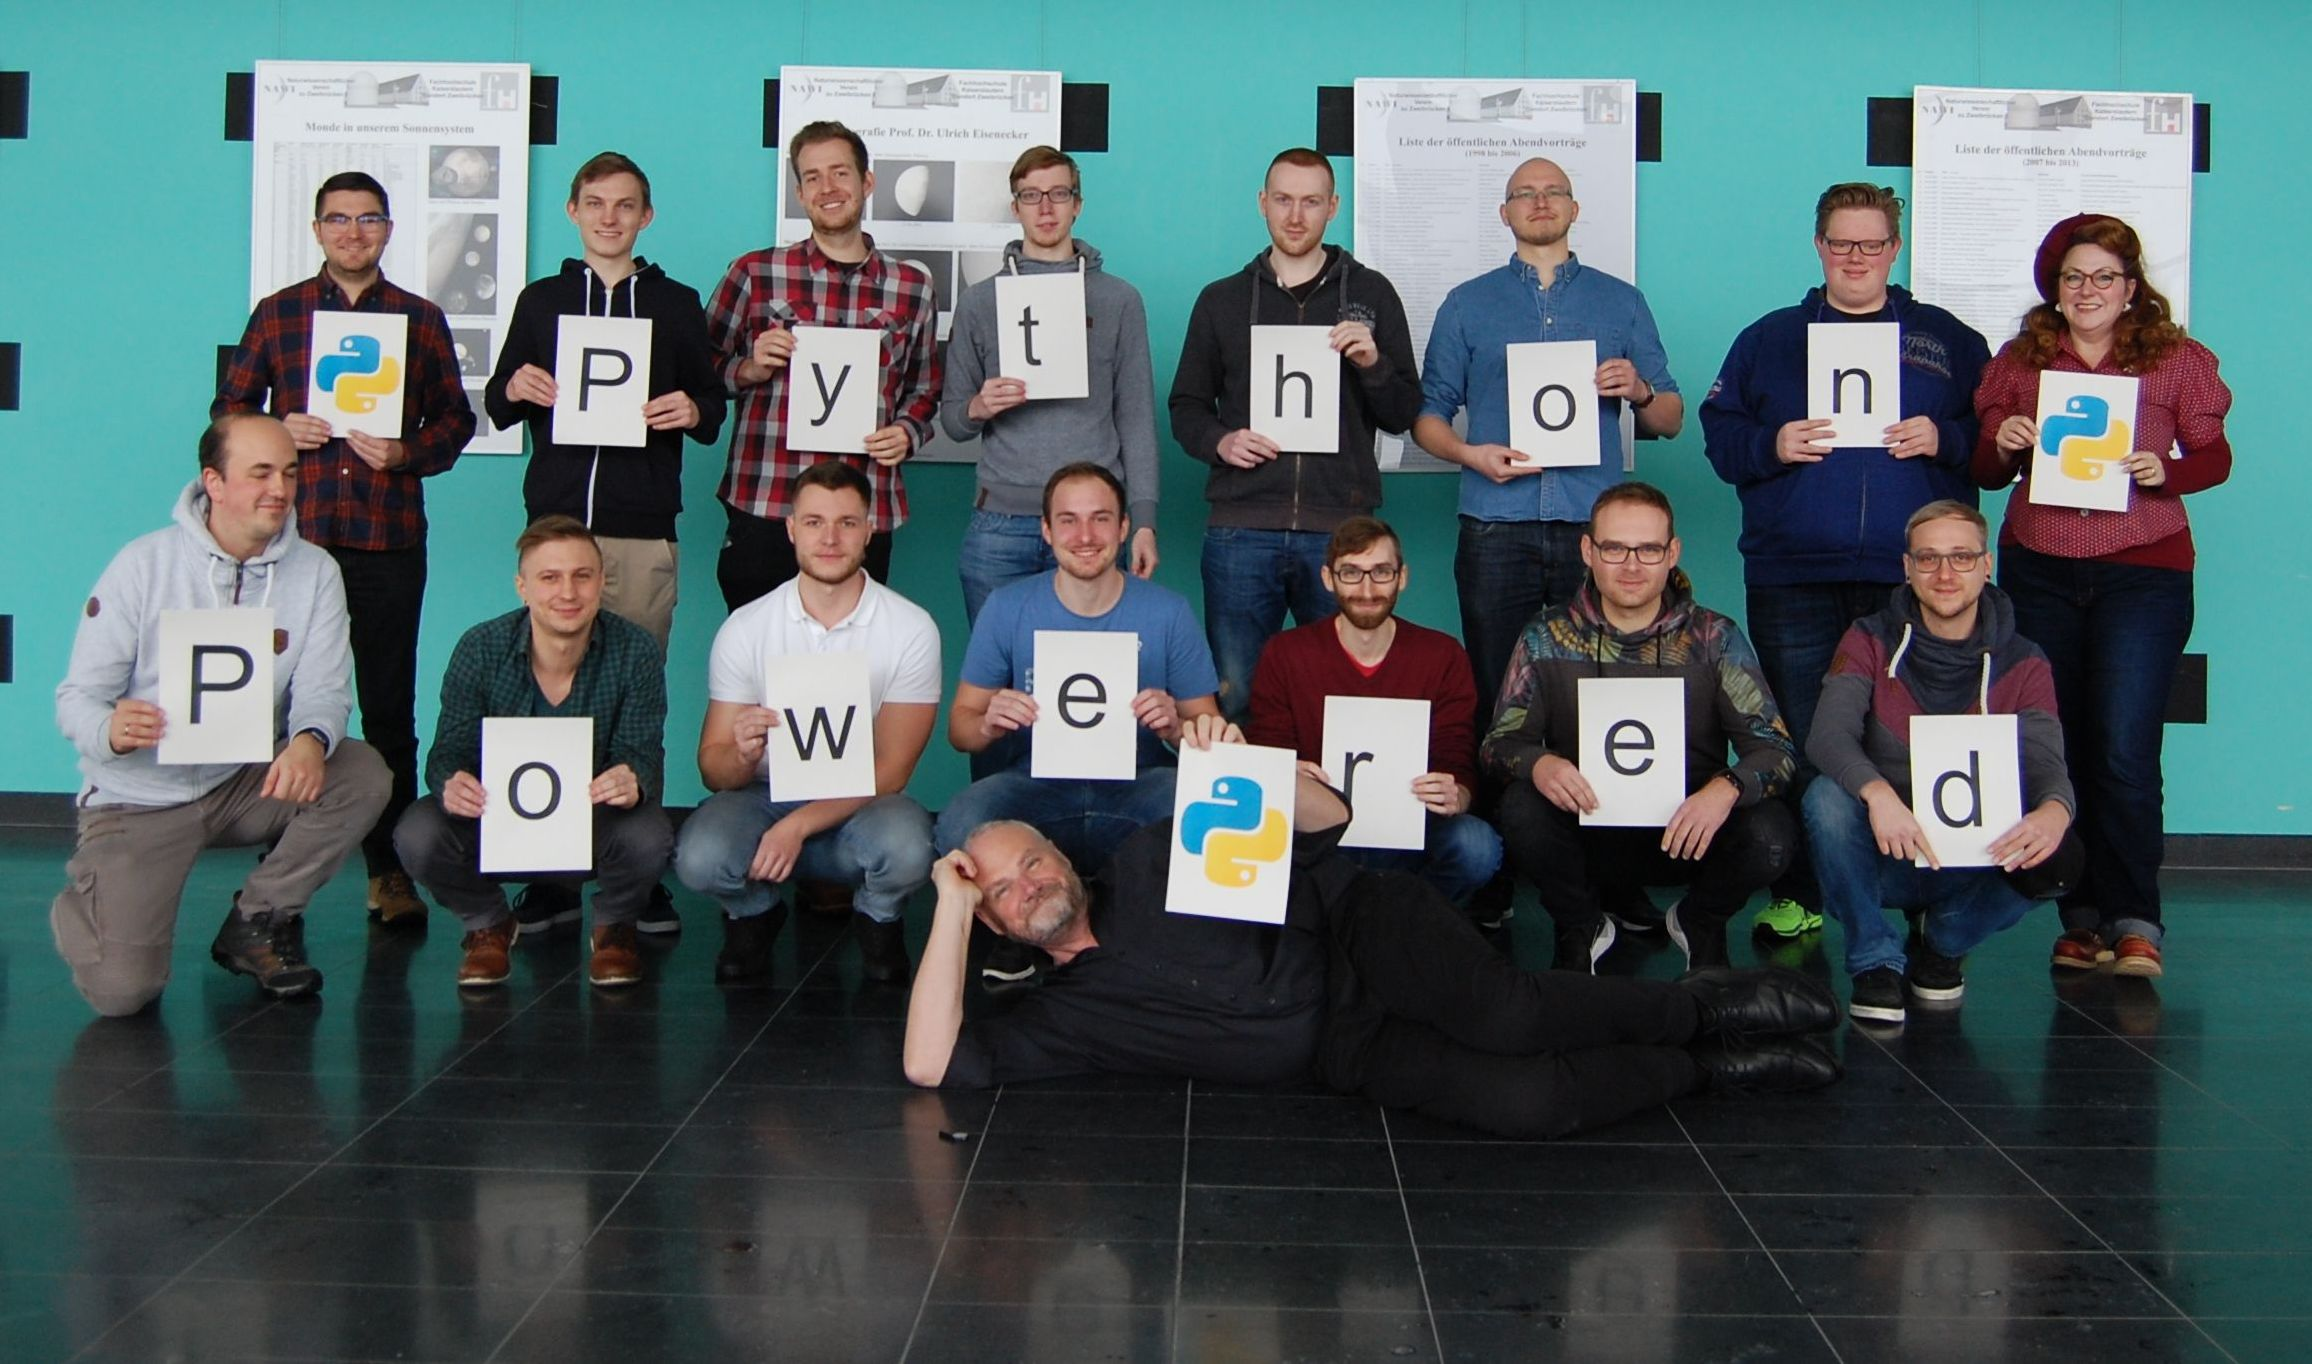
\includegraphics[width=16cm]{images/theTeam}% Rotieren mit rotate=90
%\caption{\label{vorwort:team}Das Projektteam}
\end{figure}
\begin{tabular}{ll}\hline
\centering
&Das Projektteam nach dem letzten Sprint Meeting\\
&von links nach rechts:\\\hline
Hintere Reihe&Fabian Kalweit, Matthias Haselmaier, Marc Zintel,\\
                   &Robin Guth, Anatoli Sch�fer, Denis Schlusche,\\
                   &Kevin Konrad, Miriam Lohm�ller \\\hline
Vordere Reihe&Mathias Fedder, Rainer Haffner, \ldots, Sebastian Morsch,\\
                   &Julian Bernhart, Phillip Lauer, Christoph Seibel\\\hline
Ganz vorne&Manfred Brill\\\hline
\end{tabular}
